\documentclass[a4paper,12pt,fleqn]{article}%fleqn pour aligner les equations à gauche
\usepackage{../../Styles/Cours}


\newcommand{\chnum}{Chapitre 3}
\newcommand{\chtitle}{Oxydo-réduction}
\newcommand{\dtype}{TP}
  
  
\begin{document}
\maketitle
\section*{Partie 1 : Le zinc, métal présent en construction}
\begin{minipage}{.79\linewidth}
    Le zinc est avant tout connu pour sa présence sur les toitures, notamment sur les immeubles à Paris, recouverts d'un toit en zinc, ou encore les goutières et descentes d'eau. Ce matériau trouve, depuis peu, une utilisation en tant que revêtement de façade. Apportant une apparence unique dans ses teintes, le zinc est, dans le même temps, d'une résustance incomparable.
\end{minipage}
\begin{minipage}{.2\linewidth}
    \centering
    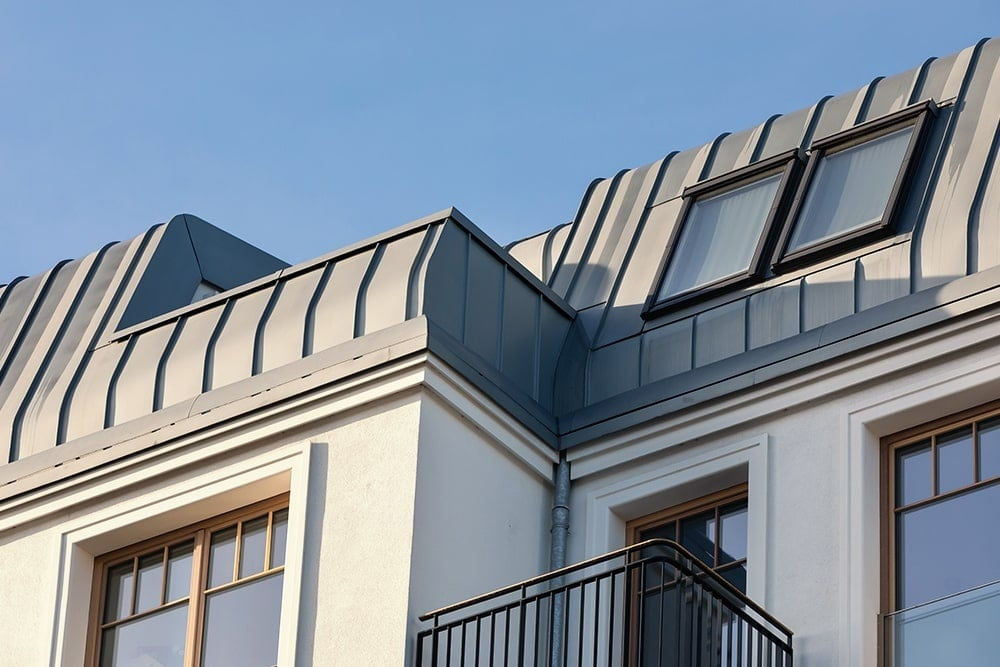
\includegraphics[width=\linewidth]{Ressources/1SPE_C03_toiture_zinc.jpg}
\end{minipage}

L'objectif de l'activité est de définir et comprendre les termes "oxydant", "réducteur", "oxydation" et "réduction".

\begin{figure}[h!]
    \begin{minipage}{.49\linewidth}
        \caption{Informations}
    L'ion zinc \ce{Zn^2+}, en présence de soude (\ce{Na+(aq), \ce{HO-(aq)}}) donne un précipité blanc d'hydroxyde de zinc \ce{Zn(OH)2(s)}.\\
    Le cuivre métallique \ce{Cu(s)} est de couleur rouge.
    \end{minipage}
    \begin{minipage}{.49\linewidth}
        \caption{Matériel mis à disposition}
        \begin{itemize}
            \item 6 tubes à essai + 2 bouchons,  Entonoir + 2 filtres, Spatule, Bécher
            \item Soude à \SI{0,1}{\mole\per\liter}
            \item Solution \ce{Cu^2+}, \ce{SO4^2-} à \SI{0,1}{\mole\per\liter} et \SI{2}{\mole\per\liter} au bureau
            \item Pastilles et poudre de zinc
        \end{itemize}
    \end{minipage}
\end{figure}

\begin{figure}[h!]
    \caption{Réaction entre le zinc métallique et les ions cuivre}
    %\begin{minipage}{.49\linewidth}
        \textbf{Protocole 1 : }
        Introduire dans un tube à essai 1 pastille de zinc \ce{Zn} et 1 mL de solution de sulfate de cuivre (\ce{Cu^2+}, \ce{SO4^2-}) à \SI{2}{\mole\per\liter}.
    %\end{minipage}
    %\begin{minipage}{.49\linewidth}
    \vspace{2em}

        \textbf{Protocole 2 :}\\
        \emph{Partie 1 :} \\
        Introduire, dasn un tube à essai, une spatule de poudre de zinc et \SI{2}{mL} de solution de sulfate de cuivre à \SI{0,1}{\mole\per\liter}.\\
        Boucher et agiter la solution.\\
        Laisser décanter puis filtrer la solution à l'aide d'un entonoir dans un bécher.\\
        Verser le filtrat dans un tube à essai.\\
        \emph{Partie 2 :}\\
        Ajouter dans le filtrat quelques gouttes de soude.
    %\end{minipage}
\end{figure}

    \subsection{Etude expérimentale : Mise en évidence de l'échange de particules}
    \begin{enumerate}
        \item Réaliser le protocole 1. Noter les observations
        \item Réaliser le protocole 2 Partie 1. Noter les observations.
        \item Réaliser le protocole 2 Partie 2. Noter les pobservations.
        \item Conclure sur le produit formé dans la \emph{Partie 1}.
    \end{enumerate}
    \subsection{Exploitation des expériences identiques (protocoles 1 et 2)}
    \begin{enumerate}[resume]
        \item Utiliser les résultats des observations pour établir un bilan des éléments zinc et de l'élément cuivre avant et après la transformation et compléter le tableau suivant :\\
        \begin{tabular}{|c|c|c|}
            \hline
            &Avant transformation & Après transformation\\
            \hline
            Espèce chimique contenant l'élément zinc & & \\
            \hline
            Espèce chimique contenant l'élément cuivre & & \\
            \hline
        \end{tabular}
    \end{enumerate}
    
    \begin{enumerate}[resume]
        \item Ecrire l'équation de la réaction chimique qui a lieu.
        \item Lors de la réaction chimique :
        \begin{enumerate}
            \item Quelle espèce chimique a perdu des électrons ? C'est un \emph{REDUCTEUR}
            \item Quelle espèce chimique a capté des électrons ? C'est un \emph{OXYDANT}
        \end{enumerate}
        \item Quel est le type de particules échangées lors de cette réactions ? C'est une réaction d'\emph{oxydoréduction}.
    \end{enumerate}
    \subsection{Définitions}
    \begin{enumerate}[resume]
        \item Compléter le texte suivant :
    \begin{cours}
        \begin{itemize}
            \item Un \hspace{5em} est une espèce chimique capable de céder un ou plusieurs électrons.
            \item Un \hspace{5em} est une espèce chimique capable de capter un ou plusieurs électrons.
            \item Un couple oxydant/réducteur est l'association de l'\hspace{5em} et du \hspace{5em} d'une même espèce.
        \end{itemize}
    \end{cours}
        \item Noter les deux couples \textbf{Ox/Red} en présence.
        \item À chaque couple est associé une demi-équation électrique : \ce{Ox + n e- = Red}
        \item Écrire les deux demi-équations électriques en plaçant le réactif à gauche.
        \item Quand on met en contact l'oxydant 1 d'un couple \ce{Ox_1}/\ce{Red_1} avec le réducteur 2 d'un couple \ce{Ox_2}/\ce{Red_2}, il peut se produire une réaction d'oxydoréduction avec transfert d'électrons : \ce{Ox_1 + Red_2 -> Red_1 + Ox_2}. Écrire l'équation de la réaction étudiée. 
    \end{enumerate}

\newpage
\section*{Partie 2 : L'arbre de Diane}
\begin{figure}[h!]
    \caption{Informations}
    Un fil de cuivre est plongé dans une solution de notrate d'argent. Il se coubre rapidement de petits filaments (dendrites) gris-blanc aussi appelés "végétation métallique". Alors que la quantité de dendrites augmente, le liquide prend une couleur bleu-ciel.
\end{figure}
\begin{figure}[h!]
    \caption{Matériel mis à disposition}
    Solution d nitrate d'argent à \SI{0,05}{\mole\per\liter}, fil de cuivre épais, tube à essai
\end{figure}
\begin{enumerate}
    \item Identifier les espèces chimiques présentes à l'état initial et à l'état final.
    \item Les ions nitrate interviennent-ils dan sla transformation chimique ? Comment se nomme ce type d'ions ?
    \item Cette transformation chimique est une oxydoréduction. L'élément oxygène intervient-il au cours de la réaction ?
    \item Concernant l'élément cuivre :
    \begin{enumerate}
        \item Sous quelle forme se trouve le cuivre à l'état innitial et à l'état final ?
        \item Proposer une demi-équation mettant en jeu l'échange d'électrons.
        \item Est-ce une oxydation ou une réduction ?
        \item Dans cette demi-équation, quel est l'oxydant et quel est le réducteur ?
    \end{enumerate}
    \item Reprendre la quastion 4. pour l'élément argent.
    \item A l'aide des deux demi-équations, écrire l'équation de la réaction étudiée.
\end{enumerate}
\end{document}
